\chapter{Results \& Discussion}
This chapter offers a detailed and thorough account of the research outcomes, emphasising their significance and the invaluable insights they bring to the forefront. The results and discussions have been meticulously structured into three key sections to maintain clarity and facilitate a comprehensive understanding of the research findings while adhering to the original formatting.

The initial section of this chapter is dedicated to the critical task of generating various query variations and systematically evaluating their validity. This is a crucial step in the research as it directly addresses our primary research questions. Crafting and assessing these query variations sheds light on the intricate methodology behind them.

The subsequent two sections are categorised in alignment with the research questions they aim to answer. The second section revolves around an in-depth analysis of the primary experiments conducted in the original study, specifically concerning the robustness of the retrieval pipelines in the face of these query variations. The outcomes and implications of reproducing the original study's main experiments are scrutinised, offering a comprehensive evaluation of the retrieval pipelines' resilience to these query variations.

The third section is dedicated to the exploration of the second research question. Here, investigation is extended by delving into the effects of query variations on an additional dataset known as DL-TYPO. This in-depth analysis allows us to draw insightful comparisons and contrasts, shedding light on how query variations impact different datasets, thus broadening the scope of our research and offering a richer perspective.

\section{Assessment of Generator Quality}
Due to the automated nature of query generation methods, the quality of the generated query variations is a focal point of this research. This emphasis on validity is rooted in the need for query variations to reflect real-world user behaviour and information needs accurately. Valid variations ensure that the experiments conducted in retrieval studies maintain authenticity that mirrors the diverse ways users express their queries. Inaccurate or invalid query variations can lead to misleading results, hindering the reliability and relevance of the research outcomes. Hence, only valid variations are used in the experiments and evaluation processes. 

A thorough evaluation of the generated query variations' quality was carried out, involving manual annotations for 1,371 pairs of {original query, developed query variation} extracted from the test sets of TREC-DL-2019, ANTIQUE and DL-TYPO. This rigorous quality assessment aimed to select only those query variations that align with the intended query variation categories, enhancing the overall reliability of the study's findings. For the sake of consistency with the original study, each pair of the ANTIQUE dataset was re-evaluated and compared to the judgements made by the original authors.

This approach was meticulously followed in this study when analysing the variations generated for the DL-TYPO dataset. This dataset comprises 60 queries, with each query undergoing query variation generation. The methods employed for query variation generation were consistent with those of the original study, albeit with minor adjustments due to the absence of sourcing from IR\_datasets. The process can be briefly summarised as follows:

\begin{enumerate}
\item \textbf{Query Variations Generation:} Following the methodology utilised in the original study, a query variation, denoted as $q\sp{\prime}$, was generated for each query, q, using each method, M (\eq{eq1}).

\begin{equation}\label{eq1}
    q\sp{\prime} = M(q)
\end{equation}

\item \textbf{Variation Editing:} Punctuation and capital letters were consistently eliminated from the query variations, adhering to the procedures delineated in the original study.
\item \textbf{Automatic Annotation:} All variations resulting from misspelling and ordering were automatically categorised as valid, as these transformations are considered rule-based and maintain the same query semantics. Additionally, any transformations leading to a query identical to the input query (\eq{eq2}) were automatically classified as invalid.

\begin{equation}\label{eq2}
    q\sp{\prime} = M(q) = q
\end{equation}

\item \textbf{Manual Annotation:} For the remaining 320 query-variation pairs, manual annotation was conducted, following criteria analogous to those employed in the original study. These criteria encompassed two primary considerations: (I) Whether qˆ retained the same semantics as q and (II) Whether the syntax difference between q and qˆ could be attributed to category C \cite{penha2022}.
\end{enumerate}

Furthermore, the observations arising from DL-TYPO variation annotations indicated several parallels with the original study, as well as novel insights:

\subsection{Parallel Findings (RQ1):}
\begin{itemize}
    \item[(I)] \textbf{T5DescToTitle Effects:} The T5DescToTitle method occasionally resulted in the removal of essential query terms, thereby altering query semantics (e.g. "things to do when broed" to "broeding" (T5DescToTitle), "how money does the show seinfled make" to "seinfled money" (T5DescToTitle)) (total of 5 occurrences).
    \item[(II)] \textbf{Replicating Identical Queries:} The BackTranslation and T5QQP methods were found to generate identical copies of the input query, which were automatically labelled as invalid (a total of 56 occurrences).
    \item[(III)] \textbf{Inaccurate Synonym Replacements:} Transformations that replaced words with presumed synonyms, such as WordEmbedSynSwap and WordNetSynSwap, sometimes introduced words that were not synonymous in the query context (e.g. "how do i clean my computor monitor screen" to "how do i clean my computor supervises screen" (WordEmbedSynSwap), "what kind of medicine is zytec" to "what kind of music is zytec" (WordNetSynSwap)). (total of 24 occurrences).
\end{itemize}
\subsection{Novel Findings (RQ2):} \label{sec:novelFindings}
\begin{itemize}
    \item[(IV)] \textbf{Proper Noun Alterations:} An expansion of the previous observation revealed that transformations occasionally replaced proper nouns or titles, causing them to no longer refer to the correct entity (e.g. "facts about chirs brown" to "facts about chirs chocolate-brown" (WordNetSynSwap), "singer axel rose" to "singer axel soars" (WordEmbedSynSwap)) (total of 11 occurrences).
    \item[(V)] \textbf{Substituting Non-English Words:} WordEmbedSynSwap replaced a word with its equivalent in another language (e.g. "flee market buildings" to "flee mercado buildings" (WordEmbedSynSwap)). This does not occur in the other datasets (total of 1 occurrence).
    \item[(VI)] \textbf{Misspelling Compounding:} Synonym and paraphrasing-related methods were observed to compound misspellings, generating queries with different semantics, despite the method functioning correctly (e.g. "medal taste in mouth symptoms" to "decoration taste in mouth symptoms" (WordNetSynSwap), "flee market buildings" to "the escape market building" (BackTranslation)) (total of 14 occurrences).
    \item[(VII)] \textbf{Fixing Spelling Errors:} Interestingly, five of the ten query variation methods were identified as fixing the original spelling errors (e.g. "alchol and drug rehab" to "alcohol and drug rehabilitation" (BackTranslation), "car accident lawers" to "what are car accident lawyers" (T5QQP), "los angelel unified school district" to "los angeles unified school" (T5DescToTitle)). BackTranslation was the method most often responsible for this correction (occurring 14 times), as well as T5QQP (7 times) (total of 25 occurrences). 
\end{itemize}

\begin{table}[ht]
\centering
\caption{Total number of valid query variations and percentage of valid variations compared to the total queries for dataset and generation method, categorised by the category.}
\label{tab:valid-vars}
\begin{tabularx}{\columnwidth}{X|r|r|r}
\textbf{Method}  & \textbf{DL-TYPO}    & \textbf{ANTIQUE}   & \textbf{TREC-DL-2019} \\ \hline
NeighbCharSwap   & 60 (100\%)          & 199 (100\%)        & 43 (100\%)            \\
RandomCharSub    & 59 (98\%)           & 197 (98\%)         & 42 (98\%)             \\
QWERTYCharSub    & 60 (100\%)          & 182 (91\%)         & 42 (98\%)             \\ \hline
RemoveStopWords  & 40 (67\%)           & 199 (100\%)        & 37 (86\%)             \\
T5DescToTitle    & 42 (70\%)           & 136 (68\%)         & 35 (81\%)             \\ \hline
RandomOrderSwap  & 60 (100\%)          & 200 (100\%)        & 43 (100\%)            \\ \hline
BackTranslation  & 34 (57\%)           & 93 (46\%)          & 23 (53\%)             \\
T5QQP            & 52 (87\%)           & 105 (52\%)         & 26 (60\%)             \\
WordEmbedSynSwap & 41 (68\%)           & 124 (62\%)         & 27 (63\%)             \\
WordNetSynSwap   & 29 (48\%)           & 71 (36\%)          & 16 (37\%)             \\ \hline
\textbf{Total}   & \textbf{477 (80\%)} & \textbf{1506 (75\%)} & \textbf{334 (78\%)}     \\ \hline
\end{tabularx}%
\end{table}


After rigorous manual annotation, 477 valid query-variation pairs for the DL-TYPO dataset were identified and retained for further analysis. These pairs were meticulously scrutinised based on their semantic integrity and alignment with the original query, providing valuable insights into the effectiveness and challenges posed by various query variation methods. The summarised results of this annotation process for all three datasets, as presented in Table \ref{tab:valid-vars}, offer valuable insights into the performance of ten query variation methods across the three distinct datasets.

In evaluating the validity of query variations, methods such as RandomOrderSwap, NeighbCharSwap, and QWERTYCharSub consistently demonstrated their robustness by producing 100\% valid variations for the DL-TYPO and ANTIQUE datasets, reflecting their capacity to create semantically coherent queries. They also performed notably well in the TREC-DL-2019 dataset, particularly QWERTYCharSub, which achieved a slightly lower but still respectable success rate of 97.7\%. RandomCharSub exhibited high percentages of valid variations, reaching 98.3\% for DL-TYPO, 98.5\% for ANTIQUE, and 97.7\% for TREC-DL-2019. 

On the other hand, RemoveStopWords displayed variable results, with a lower success rate of 66.7\% for DL-TYPO but consistently high rates of 99.5\% for ANTIQUE and 86.0\% for TREC-DL-2019. T5DescToTitle showed moderate performance, with a success rate of 70\% for DL-TYPO, 68\% for ANTIQUE, and a more promising 81.4\% for TREC-DL-2019. WordEmbedSynSwap, T5QQP, and BackTranslation exhibited varying degrees of success across datasets, with moderate rates of valid variations. In contrast, WordNetSynSwap consistently produced the lowest percentage of valid variations across all datasets, highlighting substantial challenges in generating semantically valid query variations through this method.

It is essential to acknowledge that variations in the validity of DL-TYPO annotations can be attributed, to some extent, to the change in the annotator's identity. The consistency and reliability of these annotations could be enhanced by adopting the original study's practice of involving multiple annotators for this task. Utilising multiple annotators helps mitigate potential individual annotator biases and contributes to a more comprehensive and well-rounded assessment of the dataset's quality and reliability. This approach aligns with established best practices in dataset curation, ensuring that the dataset remains a robust and valuable resource for research.
\section{Robustness to Query Variations}
\subsection{Research Question 1: Reproduction}
A comprehensive set of experiments was conducted using the same datasets, models, and methodologies to evaluate the robustness of retrieval pipelines to query variations and investigate the extent to which the original study's findings can be successfully reproduced. The key results of the reproduction study are presented in this section.

The first objective was to assess the robustness of different ranking models to query variations, categorised into lexical traditional models (Trad), neural ranking models (NN), and transformer-based language models (TNN). The effectiveness of these models, when original queries were replaced with their corresponding query variations, was determined. The results are outlined in \tab{tab:ant-main-table} for ANTIQUE and in \tab{tab:trec-main-table} for TREC-DL-2019. These tables display the resulting nDCG@10 value for each method and model, grouped by their variation category.

\begin{table}[ht]
\centering
\caption{Effectiveness (nDCG@10) of each method and model for ANTIQUE when faced with different query variations. Bold indicates the highest values observed for each model. Subscripts, ↓/↑, signify statistically significant decreases/increases obtained through a two-sided paired Student's T-Test conducted at a 95\% confidence level when comparing the model's performance with the original queries.}
\label{tab:ant-main-table}
\resizebox{\columnwidth}{!}{%
\begin{tabular}{l|l|l|l|l|l|l|l|l}
\textbf{\textbf{Category}} & \textbf{\textbf{Variation Method}} & \textbf{\textbf{BM25}} & \textbf{\textbf{RM3}} & \textbf{KNRM} & \textbf{CKNRM} & \textbf{EPIC} & \textbf{BERT} & \textbf{T5} \\ \hline
- & Original Query & \textbf{0.2286} & \textbf{0.217} & 0.2181 & 0.2065 & 0.266 & \textbf{0.363} & \textbf{0.3333} \\ \hline
Misspelling & NeighbCharSwap & 0.1559↓ & 0.1469↓ & 0.159↓ & 0.1444↓ & 0.184↓ & 0.2608↓ & 0.2509↓ \\
Misspelling & QWERTYCharSub & 0.1613↓ & 0.1525↓ & 0.162↓ & 0.1553↓ & 0.192↓ & 0.2619↓ & 0.2652↓ \\
Misspelling & RandomCharSub & 0.1623↓ & 0.1593↓ & 0.1602↓ & 0.1476↓ & 0.1879↓ & 0.2563↓ & 0.2458↓ \\ \hline
Naturality & RemoveStopWords & 0.227 & 0.2161 & \textbf{0.2232} & \textbf{0.2153} & \textbf{0.2693} & 0.3391↓ & 0.32 \\
Naturality & T5DescToTitle & 0.1673↓ & 0.1646↓ & 0.1647↓ & 0.1672↓ & 0.2006↓ & 0.2402↓ & 0.2393↓ \\ \hline
Ordering & RandomOrderSwap & \textbf{0.2286} & 0.2169 & 0.2181 & 0.1978 & 0.2661 & 0.3566 & 0.3255 \\ \hline
Paraphrase & BackTranslation & 0.1618↓ & 0.1546↓ & 0.1609↓ & 0.1438↓ & 0.2032↓ & 0.274↓ & 0.2581↓ \\
Paraphrase & T5QQP & 0.2201 & 0.2063 & 0.2085 & 0.1957 & 0.2617 & 0.3389↓ & 0.3214 \\
Paraphrase & WordEmbedSynSwap & 0.1759↓ & 0.1715↓ & 0.1915↓ & 0.1689↓ & 0.2139↓ & 0.2809↓ & 0.2814↓ \\
Paraphrase & WordNetSynSwap & 0.1791↓ & 0.175↓ & 0.1933↓ & 0.1763↓ & 0.212↓ & 0.2829↓ & 0.2734↓ \\ \hline
\end{tabular}%
}
\end{table}
\begin{table}[ht]
\centering
\caption{Effectiveness (nDCG@10) of each method and model for TREC-DL-2019 when faced with different query variations. Bold indicates the highest values observed for each model. Subscripts, ↓/↑, signify statistically significant decreases/increases obtained through a two-sided paired Student's T-Test conducted at a 95\% confidence level when comparing the model's performance with the original queries.}
\label{tab:trec-main-table}
\resizebox{\columnwidth}{!}{%
\begin{tabular}{l|l|l|l|l|l|l|l|l}
\textbf{Category} & \textbf{Variation Method} & \textbf{BM25} & \textbf{RM3} & \textbf{KNRM} & \textbf{CKNRM} & \textbf{EPIC} & \textbf{BERT} & \textbf{T5}  \\ \hline
- & Original Query    & \textbf{0.4795} & \textbf{0.5156} &\textbf{ 0.4941} & \textbf{0.4931} & \textbf{0.624}  & \textbf{0.6358} & 0.6998  \\ \hline
Misspelling     & NeighbCharSwap   & 0.2747↓ & 0.2748↓ & 0.3078↓ & 0.308↓  & 0.3893↓ & 0.3812↓ & 0.4944↓ \\ 
Misspelling     & QWERTYCharSub    & 0.2435↓ & 0.2504↓ & 0.2563↓ & 0.2965↓ & 0.3496↓ & 0.3657↓ & 0.4461↓ \\ 
Misspelling     & RandomCharSub    & 0.2314↓ & 0.2347↓ & 0.2349↓ & 0.2263↓ & 0.295↓  & 0.3075↓ & 0.3963↓  \\ \hline
Naturality      & RemoveStopWords  & 0.4778 & 0.5113 & 0.4769 & 0.4756 & 0.6214 & 0.615  & 0.6862  \\ 
Naturality      & T5DescToTitle    & 0.4215 & 0.4344 & 0.3693↓ & 0.3928 & 0.5061↓ & 0.533↓  & 0.5717↓ \\ \hline
Ordering        & RandomOrderSwap  & \textbf{0.4795} & \textbf{0.5156} & \textbf{0.4941} & 0.4708 & 0.6227 & 0.6268 & 0.697  \\ \hline
Paraphrase      & BackTranslation  & 0.3964 & 0.4195 & 0.3954 & 0.3605↓ & 0.5301 & 0.4874↓ & 0.6058 \\ 
Paraphrase      & T5QQP            & 0.4722 & 0.5043 & 0.4525 & 0.4609 & 0.604  & 0.6222 & \textbf{0.7045} \\ 
Paraphrase      & WordNetSynSwap   & 0.3488↓ & 0.365↓  & 0.3615↓ & 0.3605↓ & 0.449↓  & 0.459↓  & 0.5457↓ \\ 
Paraphrase      & WordEmbedSynSwap & 0.353↓  & 0.3539↓ & 0.3767↓ & 0.368↓  & 0.4749↓ & 0.4816↓ & 0.5603↓  \\ \hline
\end{tabular}%
}
\end{table}

The findings reveal a substantial degree of alignment with the original study. The experiments consistently demonstrate a statistically significant decline in retrieval effectiveness when various query variations and model combinations are considered. For the TREC-DL-2019 dataset, this reduction is observed in 41 out of 70 instances, representing a slight deviation from the original study's results by 8 cases. Similarly, for the ANTIQUE dataset, a decrease in effectiveness is recorded in 51 instances, deviating by merely 3 cases from the original study's outcomes. Furthermore, the analysis of valid queries illustrates that, on average, the models experience a reduction in effectiveness of 22.02\% for TREC-DL-2019, a figure marginally distinct from the original study's 20.62\%. For ANTIQUE, the average decline amounts to 17.92\%, contrasting with the original study's 19.21\%. These consistent trends reaffirm the original study's pivotal assertion that retrieval pipelines exhibit limited robustness in the face of query variations. These outcomes substantiate previous evidence suggesting that query variations introduce considerable variability into diverse information retrieval systems.

Discrepancies emerge when comparing specific values between this study and the original research. On average, the discrepancies are less than 0.08; however, they are particularly evident in the results for the BERT model. One potential explanation for these differences is the value of training iterations. Although the exact training iteration value used in the original study remains undisclosed, when reproducing the study, a value of only 50 was used due to computational constraints. Notably, these minor deviations in results underline the intricate nature of replication work, where subtle variations in experimental settings, environmental conditions, or data pre-processing procedures can lead to distinctions in experimental outcomes.

The replication study effectively addresses Research Question 1 (RQ1). Through a meticulous replication of experiments and methodologies from the original study, critical insights have been offered, and the original findings fortified. The consistently corroborated results from the reproduction study underscore the limited robustness of retrieval pipelines in the face of query variations, consequently reinforcing the pivotal conclusion of the original study. This coherence in findings between the two independent studies signifies the robustness and broader applicability of the original study's observations. This outcome robustly attests to the validity of the research outcomes in the original study's context and their broader relevance, accentuating the significant role of query variations in evaluating retrieval systems.

\subsection{Research Question 2: Expansion}
To assess the generalisability of the original findings, the study replicated the experiments using the DL-TYPO dataset. Moreover, as the original study suggested that neural ranking models might not handle query variations well, even with modern datasets, DL-TYPO emerged as an apt candidate for testing the transference of this inquiry. The selection of DL-TYPO was motivated by its novel and unexplored nature, thereby substantiating its suitability for broadening the research.

\begin{table}[ht]
\centering
\caption{Effectiveness (nDCG@10) of each method and model for DL-TYPO when faced with different query variations. Bold indicates the highest value observed for each model. Subscripts, ↓/↑, signify statistically significant decreases/increases obtained through a two-sided paired Student's T-Test conducted at a 95\% confidence level when comparing the model's performance with the original queries.}
\label{tab:typo-main-table}
\resizebox{\columnwidth}{!}{%
\begin{tabular}{l|l|l|l|l|l|l|l|l}
\textbf{Category} & \textbf{Variation Method} & \textbf{BM25} & \textbf{RM3} & \textbf{KNRM} & \textbf{CKNRM} & \textbf{EPIC} & \textbf{BERT} & \textbf{T5} \\ \hline
- & Original Query    & 0.1911 & 0.1757 & \textbf{0.2117} & \textbf{0.1798} & 0.1862 & 0.1951↓ & 0.2882 \\ \hline
Misspelling     & NeighbCharSwap   & 0.1145 & 0.1086 & 0.1224↓ & 0.0961↓ & 0.0987↓ & 0.0865↓ & 0.1922  \\
Misspelling     & QWERTYCharSub    & 0.0772↓ & 0.0746↓ & 0.0813↓ & 0.0572↓ & 0.0707↓ & 0.0683↓ & 0.1139↓  \\
Misspelling     & RandomCharSub    & 0.068↓  & 0.0626↓ & 0.1083↓ & 0.079↓  & 0.0844↓ & 0.0733↓ & 0.148↓  \\ \hline
Naturality      & RemoveStopWords  & 0.1911 & 0.1757 & 0.2022 & 0.1666 & 0.1825 & 0.1762 & 0.2794  \\
Naturality      & T5DescToTitle    & 0.1347 & 0.1244 & 0.1351↓ & 0.1228 & 0.1434 & 0.1454 & 0.2055  \\ \hline
Ordering        & RandomOrderSwap  & 0.1911 & 0.1757 & \textbf{0.2117} & 0.1443 & 0.1875↓ & 0.1719 & 0.2707  \\ \hline
Paraphrase      & BackTranslation  & 0.1468 & 0.141  & 0.1578 & 0.121  & 0.1702 & 0.1625 & 0.2245  \\
Paraphrase      & T5QQP            & \textbf{0.2138} & \textbf{0.2052} & 0.1738 & 0.1546 & \textbf{0.1956} & \textbf{0.218} & \textbf{0.2897}  \\
Paraphrase      & WordEmbedSynSwap & 0.0809 & 0.075  & 0.106↓  & 0.0901↓ & 0.0976↓ & 0.0638↓ & 0.1326↓  \\
Paraphrase      & WordNetSynSwap   & 0.1097↓ & 0.0978↓ & 0.1255↓ & 0.1004↓ & 0.1033↓ & 0.1018↓ & 0.1726↓ \\ \hline
\end{tabular}%
}
\end{table}

\tab{tab:typo-main-table} displays the results for DL-TYPO when applying the same models and methodologies used in the original study. This table shows the resulting nDCG@10 value for each method and model, grouped by their variation category.

The primary objective was to ascertain if the conclusions regarding retrieval pipeline robustness held when confronted with this real query dataset. As anticipated, the results closely paralleled the original research with discernibly diminished effectiveness. A pronounced reduction in the retrieval models' performance manifested across most query variation scenarios, thus substantiating the initial investigation's findings. Notably, the extent of the overall effectiveness decline, averaging at 31.81\%, surpassed that observed for TREC-DL-2019 and ANTIQUE. This observation underscores the resilience of the conclusions derived from the original study when transposed to the novel and distinct DL-TYPO dataset. The research's core inferences and insights possess a certain degree of generalisability, albeit with the caveat of nuanced dataset-specific variations in the extent of the observed effects.

The variation in results between the DL-TYPO dataset and the previously studied datasets can be attributed to several underlying factors. Firstly, the DL-TYPO dataset inherently features more query variations (misspellings, specifically) than the synthetically generated counterparts. The diversity and unpredictability of these authentic query variations pose a more substantial challenge to the robustness of retrieval pipelines, leading to a potentially higher decline in effectiveness. Furthermore, the specific characteristics of the queries in the DL-TYPO dataset, such as the frequency and types of typos, differ significantly from those in the other datasets. These idiosyncrasies interact with the retrieval models and the query variations in a distinct manner, further contributing to variations in observed effectiveness.

As mentioned in the original study, dataset-specific properties, such as query lengths, language styles, and topical diversity, play a role in the differing outcomes. Additionally, the performance of retrieval models may also be influenced by the dataset's composition in terms of judged and unjudged documents. If the query variations in the DL-TYPO dataset significantly increase unjudged documents' ranking highly, this could impact the perceived effectiveness, even if some of these documents might be contextually relevant.

In comparing the performance of retrieval models on the DL-TYPO dataset to that on the ANTIQUE and TREC-DL-2019 datasets, it becomes evident that DL-TYPO exhibits a significant reduction in effectiveness when confronted with various query variations. This underperformance of DL-TYPO can be attributed to several factors, as discussed. 

\subsection{Robustness by Query Variation Category}
The approach employed in the original study was replicated to examine the impact of different query variation categories on model effectiveness. Four distinct categories, namely misspellings, paraphrasing, naturality, and ordering, were systematically assigned to various query variations. The distribution of nDCG@10 $\Delta$ values across all models and variation categories is illustrated in the accompanying \fig{fig:dist-plots}, and these results are substantiated by the mean nDCG@10 $\Delta$ values per category and dataset, as depicted in \fig{fig:cat-changes}.

\begin{figure}[ht]
    \centering
    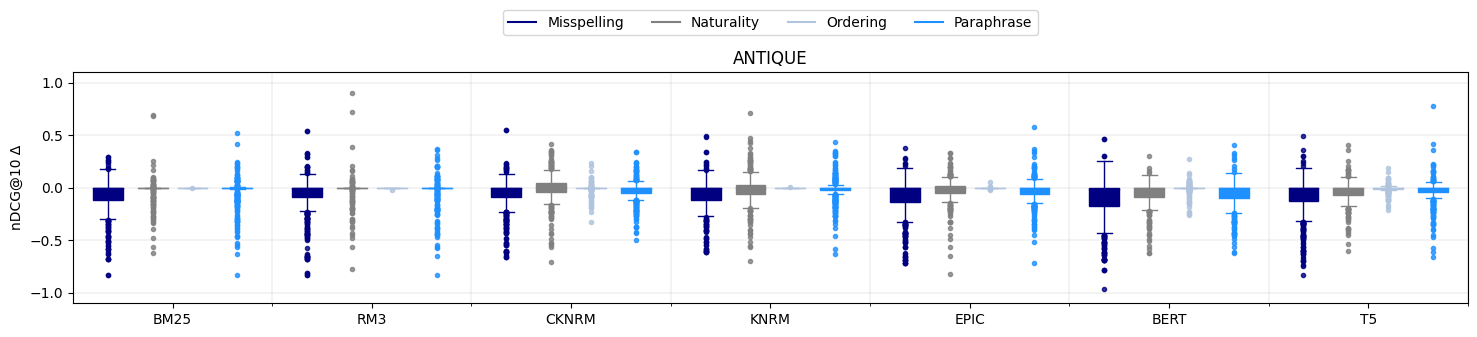
\includegraphics[width=1\linewidth]{5Results/main/plot_dist_antique.png}
    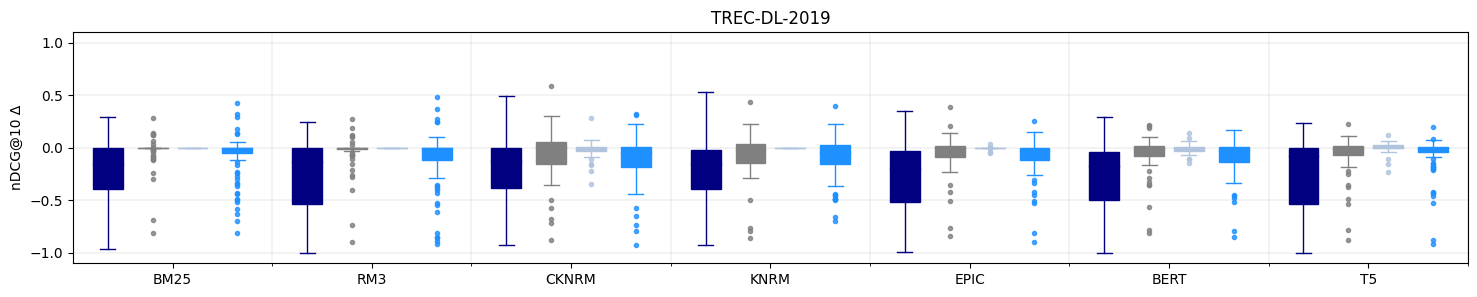
\includegraphics[width=1\linewidth]{5Results/main/plot_dist_trec.png}
    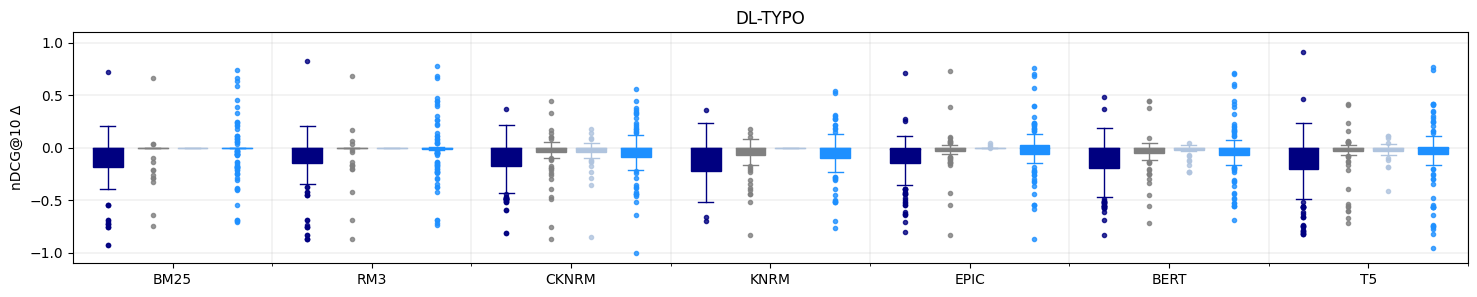
\includegraphics[width=1\linewidth]{5Results/main/plot_dist_dl-typo.png}
    \caption{Distribution of nDCG@10 $\Delta$ when replacing the original query by the methods of each category.}
    \label{fig:dist-plots}
\end{figure}

\begin{figure}[ht]
    \centering
    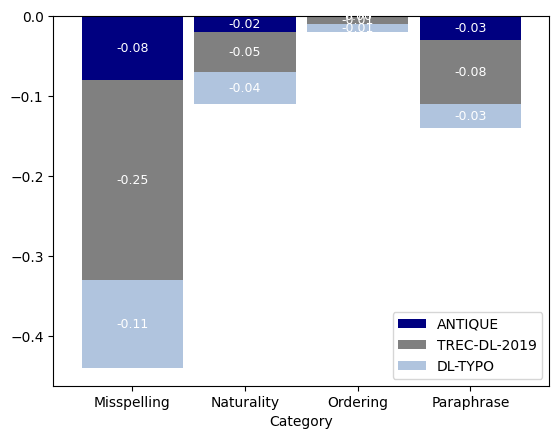
\includegraphics[width=0.8\linewidth]{5Results/main/plot_cat_changes.png}
    \caption{Average nDCG@10 $\Delta$ values per variation category for each dataset.}
    \label{fig:cat-changes}
\end{figure}

The findings highlight that, on average, the most pronounced negative impact was observed in misspelling variations. These variations recorded nDCG@10 $\Delta$ values of -0.08 for ANTIQUE, -0.25 for TREC-DL-2019, and -0.11 for DL-TYPO. These outcomes align with the observations made in the original study, further reinforcing the notion that misspelling variations consistently undermine retrieval effectiveness. In contrast, variations falling under the paraphrasing and naturality categories exhibited more modest nDCG@10 $\Delta$ values, with specific queries displaying a positive effect, mitigating the overall decline in retrieval performance. Notably, ordering variations had a negligible impact on traditional models, owing to their inherent nature as bag-of-words models, resulting in an average nDCG@10 $\Delta$ close to zero. This comprehensive evaluation elucidates the divergent impacts of distinct query variation categories on the efficacy of retrieval models. The consistent underperformance of DL-TYPO compared to ANTIQUE and TREC-DL-2019 further validates the notion that misspellings lead to diminished retrieval effectiveness. This is evident when comparing the original query values in \tab{tab:typo-main-table} with those in \tab{tab:ant-main-table} and \tab{tab:trec-main-table}.

\tab{tab:m-egs} provides an overview of how each of the methods affect the nDCG@10 $\Delta$ when applied to an example query from DL-TYPO. Notably, the T5DescToTitle method results in a significant reduction in nDCG@10 of 75\% . Other methods, such as NeighbCharSwap, RandomCharSub, and QWERTYCharSub, lead to approximately 49\% decreases in nDCG@10, underscoring their detrimental impact on query variations. This analysis emphasises the importance of carefully selecting variation methods, as their effects can vary significantly and have a substantial impact on the quality of retrieval results.

\begin{table}[ht]
\centering
\caption{Query variation and resulting change in effectiveness (nDCG@10 $\Delta$)  when we replace an example query from DL-TYPO with its variations for each variation method.}
\label{tab:m-egs}
\begin{tabularx}{\columnwidth}{l|X|l}
\textbf{Variation Method (M)} & \textbf{M("what does the declaration of independance represent")} & \textbf{nDCG@10 $\Delta$} \\ \hline
NeighbCharSwap  & what does the declaration of independance repreesnt  & -0.14 (-49.0\%) \\
RandomCharSub   & what does the declaration of independance represant  & -0.1 (-35.0\%)  \\
QWERTYCharSub   & what does the declaration of independance reprssent  & -0.14 (-49.0\%) \\ \hline
RemoveStopWords & declaration independance represent                   & -0.12 (-40.0\%) \\
T5DescToTitle   & declaration of independance                          & -0.22 (-75.0\%) \\ \hline
RandomOrderSwap & what does the declaration represent independance of  & -0.02 (-6.0\%)  \\ \hline
BackTranslation & what is the declaration of independence              & -0.14 (-49.0\%) \\
T5QQ            & what does the declaration of independence represent  & -0.05 (-17.0\%) \\
WordEmbedSynSwap    & what does the declaration of independance representing            & -0.04 (-15.0\%)           \\
WordNetSynSwap  & what does the announcement of independance represent & Invalid variation \\ \hline
\end{tabularx}%
\end{table}

\section{Fusing Query Variations}
Despite the infrequent occurrences, it is evident from the data presented in \fig{fig:dist-plots} that, in some instances, superior performance is observed for the query variations over their original counterparts. This is shown by a positive nDCG@10 $\Delta$. Following the original research, this phenomenon is the impetus for exploring the amalgamation of different query variation types.

The resulting effectiveness of merging the rankings for each variation category is illustrated in \tab{tab:ant-fusion-table}, \tab{tab:trec-fusion-table}, and \tab{tab:typo-fusion-table}. Rows denoted as $ RFC_C $ signify the amalgamation of results derived from query variations obtained by applying $ M_C $ methods using the Reciprocal Rank Fusion (RRF) technique, while $ RFC_{All} $ encompasses the results from all query variation methods. It is notable that the $ RFC_{Ordering} $ category is excluded, as it comprises only a single method.

\subsection{Research Question 1: Reproduction}
\begin{table}[ht]
\centering
\caption{Effectiveness (nDCG@10) of different methods for ANTIQUE when employing rank fusion (RRF) of the rankings obtained by using different sets of queries.}
\label{tab:ant-fusion-table}
\begin{tabularx}{\columnwidth}{l|X|X|X|X|X|X|X}
\textbf{} & \textbf{BM25} & \textbf{RM3} & \textbf{KNRM} & \textbf{CKNRM} & \textbf{EPIC} & \textbf{BERT} & \textbf{T5} \\ \hline
Original Query   & 0.2286 & 0.217  & 0.2182  & 0.2065 & 0.266  & 0.3947  & 0.3333 \\ \hline
$RRF_{Misspelling}$ & 0.1714 & 0.1653 & 0.1804  & 0.1664 & 0.2065 & 0.2675  & 0.2441 \\
$RRF_{Naturality}$  & 0.1842 & 0.1865 & 0.2058  & 0.2039 & 0.2407 & 0.3002  & 0.271  \\
$RRF_{Paraphrase}$  & 0.1924 & 0.1861 & 0.1955  & 0.1765 & 0.2401 & 0.3223  & 0.2894 \\
$RRF_{Synonym}$     & 0.1831 & 0.177  & 0.2009  & 0.1847 & 0.2184 & 0.2944  & 0.2678 \\
$RRF_{All}$         & 0.2076 & 0.206  & 0.219   & 0.2121 & 0.2547 & 0.3197  & 0.2867 \\ \hline
Best Query       & 0.4149 & 0.2716 & 0.2836  & 0.3369 & 0.3019 & 0.3981  & 0.3911
\end{tabularx}%
\end{table}

\begin{table}[ht]
\centering
\caption{Effectiveness (nDCG@10) of different methods for TREC-DL-2019 when employing rank fusion (RRF) of the rankings obtained by using different sets of queries.}
\label{tab:trec-fusion-table}
\begin{tabularx}{\columnwidth}{l|X|X|X|X|X|X|X}

\textbf{} & \textbf{\textbf{BM25}} & \textbf{\textbf{RM3}} & \textbf{KNRM} & \textbf{CKNRM} & \textbf{EPIC} & \textbf{BERT} & \textbf{T5} \\ \hline
Original Query   & 0.4795 & 0.5156 & 0.4941 & 0.4931 & 0.624  & 0.6358 & 0.6998 \\ \hline
$RRF_{Misspelling}$ & 0.3035 & 0.3073 & 0.3175 & 0.3175 & 0.3838 & 0.3941 & 0.4636 \\
$RRF_{Naturality}$  & 0.4744 & 0.4972 & 0.4668 & 0.464  & 0.5925 & 0.6005 & 0.6643 \\
$RRF_{Paraphrase}$  & 0.4742 & 0.4865 & 0.4883 & 0.433  & 0.5847 & 0.577  & 0.6616 \\
$RRF_{Synonym}$     & 0.4247 & 0.4066 & 0.4117 & 0.4048 & 0.4975 & 0.4902 & 0.5632 \\
$RRF_{All}$         & 0.4752 & 0.4958 & 0.4965 & 0.4951 & 0.5908 & 0.5939 & 0.6442 \\ \hline
Best Query       & 0.6964 & 0.5401 & 0.6116 & 0.6983 & 0.6939 & 0.6784 & 0.7598
\end{tabularx}
\end{table}

The incorporation of RRF yields significant enhancements in nDCG@10, as demonstrated in \tab{tab:ant-fusion-table} and \tab{tab:trec-fusion-table}. A comparative analysis with \tab{tab:ant-main-table} and \tab{tab:trec-main-table} reveals that, in numerous instances, the outcomes are either on par with or surpass the performance achieved through the sole utilisation of query variations. This pattern of results aligns with the original study's findings, bolstering the assertion that RRF can augment retrieval effectiveness. However, the augmentation by RRF does not consistently outperform the retrieval outcomes associated with the unaltered original queries. This observation underscores the nuanced impact of RRF within the context of query variations and retrieval performance.

\subsection{Research Question 2: Expansion}
\begin{table}[ht]
\centering
\caption{Effectiveness (nDCG@10) of different methods for DL-TYPO when employing rank fusion (RRF) of the rankings obtained by using different sets of queries.}
\label{tab:typo-fusion-table}
\begin{tabularx}{\columnwidth}{l|X|X|X|X|X|X|X}

\textbf{} & \textbf{BM25} & \textbf{RM3} & \textbf{KNRM} & \textbf{CKNRM} & \textbf{EPIC} & \textbf{BERT} & \textbf{T5} \\ \hline
Original Query   & 0.1911 & 0.1757 & 0.1994 & 0.1798 & 0.1862 & 0.1951 & 0.2882 \\ \hline
$RRF_{Misspelling}$ & 0.0979 & 0.0933 & 0.1147 & 0.0855 & 0.1006 & 0.0782 & 0.1373 \\
$RRF_{Naturality}$  & 0.1657 & 0.154  & 0.1592 & 0.1498 & 0.161  & 0.1557 & 0.2277 \\
$RRF_{Paraphrase}$  & 0.1965 & 0.1919 & 0.1839 & 0.1722 & 0.202  & 0.1931 & 0.2479 \\
$RRF_{Synonym}$     & 0.0883 & 0.0795 & 0.1214 & 0.0945 & 0.1051 & 0.0932 & 0.1477 \\
$RRF_{All}$         & 0.1546 & 0.1516 & 0.184  & 0.159  & 0.1656 & 0.156  & 0.2098 \\ \hline
Best Query        & 0.3156 & 0.3024 & 0.275  & 0.317  & 0.3052 & 0.2913 & 0.421 
\end{tabularx}
\end{table}


The effectiveness results (nDCG@10) for DL-TYPO when employing RRF are depicted in \tab{tab:typo-fusion-table}. They exhibit a noticeable disparity compared to the outcomes from ANTIQUE and TREC-DL-2019, as shown in \tab{tab:trec-fusion-table} and \tab{tab:typo-fusion-table}. DL-TYPO demonstrates lower nDCG@10 values for the original queries, indicative of a more challenging retrieval scenario. The influence of query variations and their subsequent amalgamation through RRF mirrors the results in ANTIQUE and TREC-DL-2019, as they lead to enhancements over the original queries. Nonetheless, these improvements are more modest in DL-TYPO, underscoring the unique characteristics of the dataset and the incredible difficulty in achieving substantial enhancements through query variations and RRF.

This disparity arises from the inherently more challenging nature of queries in the DL-TYPO dataset, which contain typos, resulting it it showing lower retrieval effectiveness. Consequently, the improvements stemming from query variations and RRF are less pronounced than in ANTIQUE and TREC-DL-2019. The disparities in results underscore the dataset-specific nature of this research and emphasise the significance of considering the distinct attributes and challenges of different datasets when exploring query variations and their impact on retrieval performance.

\subsection{Query Variations Performance}
\fig{fig:pos-diffs} provides visual insight into the performance of various query variation methods. The naturality and paraphrase methods exhibit more substantial improvements in variation effectiveness over the original queries compared to the other methods. Notably, the paraphrase category boasts the highest number of variations, demonstrating improved effectiveness across all models and datasets. This implies that paraphrasing query variations can outperform the original queries. The counts of such improvements range from 13 to 19, highlighting significant variability in successful paraphrased queries across models and datasets. This variance can be attributed to the propensity of paraphrasing methods to enhance queries by rectifying spelling errors (e.g. See \secn{sec:novelFindings}) and replacing words with more appropriate synonyms (e.g. "real gohst pics" to "authentic gohst pics" through WordEmbedSynSwap).
\begin{figure}
    \centering
    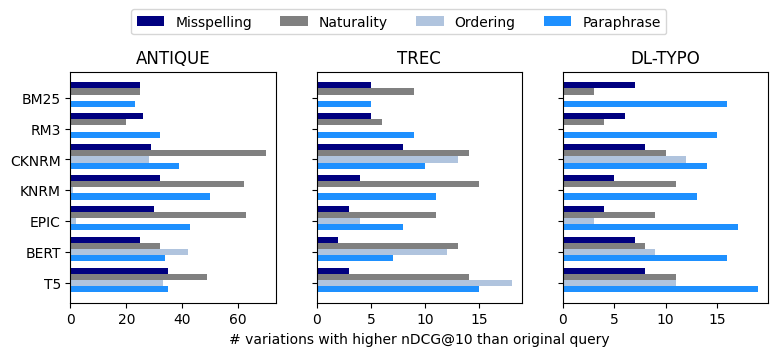
\includegraphics[width=1\linewidth]{5Results/fusion/plot_pos_diffs.png}
    \caption{Number of variations with higher effectiveness (nDCG@10) than original query per model for each variation category.}
    \label{fig:pos-diffs}
\end{figure}

In contrast, the ordering category exhibits limited variations with improved effectiveness. In some instances, such as Trad and NN on specific datasets like TREC-DL-2019 and ANTIQUE, no variations surpass the effectiveness of the original query. This can be attributed to the impact of alterations in word order on retrieval effectiveness, especially within traditional bag-of-words models. Overall, the data underscores the significance of the specific nature of query variations and their interaction with diverse retrieval models and datasets. Overall, paraphrasing variations show great promise in enhancing retrieval performance while ordering variations seem to have a restricted impact.

The data underscores the disparities in the effectiveness of query variations, particularly in DL-TYPO compared to ANTIQUE and TREC-DL-2019. DL-TYPO exhibits fewer variations with higher nDCG@10 effectiveness than the original query. This suggests that query variations have a less pronounced impact on retrieval effectiveness in DL-TYPO. The variability in the number of improvements is also conspicuous across the categories of query variations. Moreover, this variability depends on the specific retrieval model employed, with some models showing a more substantial number of successful query variations than others. These differences underscore the challenges posed by real-world queries containing typos in the DL-TYPO dataset, as opposed to the synthetic data in other datasets. These observations emphasise the need for further research to comprehend the unique challenges presented by diverse datasets when working with query variations and retrieval models.
